% ============================================================
%  Aura Budget — Beamer Presentation
%  Compile with: pdflatex presentation.tex
% ============================================================
\documentclass[aspectratio=169, 11pt]{beamer}

% ---------- Theme & Colors ----------
\usetheme{Madrid}
\usecolortheme{default}

\definecolor{auraviolet}{RGB}{124, 58, 237}
\definecolor{auradark}{RGB}{30, 15, 60}
\definecolor{auragray}{RGB}{245, 243, 255}
\definecolor{auraaccent}{RGB}{167, 139, 250}

\setbeamercolor{palette primary}{bg=auraviolet, fg=white}
\setbeamercolor{palette secondary}{bg=auradark, fg=white}
\setbeamercolor{palette tertiary}{bg=auraaccent, fg=auradark}
\setbeamercolor{palette quaternary}{bg=auradark, fg=white}
\setbeamercolor{structure}{fg=auraviolet}
\setbeamercolor{section in toc}{fg=auraviolet}
\setbeamercolor{block title}{bg=auraviolet, fg=white}
\setbeamercolor{block body}{bg=auragray, fg=auradark}
\setbeamercolor{alerted text}{fg=auraviolet}

% ---------- Packages ----------
\usepackage{booktabs}
\usepackage{graphicx}
\usepackage{fontawesome5}
\usepackage{tikz}
\usetikzlibrary{shapes.geometric, arrows.meta, positioning}
\usepackage{xcolor}
\usepackage{array}
\usepackage{tabularx}

% ---------- Font ----------
\usefonttheme{professionalfonts}
\usepackage[T1]{fontenc}

% ---------- Meta ----------
\title[Aura Budget]{\textbf{Aura Budget}}
\subtitle{An AI-Powered Personal Finance Management System}
\author{Student Research Project}
\institute{SRP Project}
\date{March 2026}

% ---------- Custom commands ----------
\newcommand{\bulletitem}[1]{\item[\textcolor{auraviolet}{\faCheckCircle}] #1}

% ============================================================
\begin{document}

% ---- Title Slide ----
\begin{frame}
  \titlepage
  \begin{center}
    \small\textcolor{auradark}{Combining AI/LLM insights, ML forecasting, and real-time
    collaboration in a modern personal finance platform.}
  \end{center}
\end{frame}

% ---- Table of Contents ----
\begin{frame}{Outline}
  \tableofcontents
\end{frame}

% ============================================================
\section{Introduction}
% ============================================================
\begin{frame}{Introduction}
  \begin{columns}[T]
    \begin{column}{0.55\textwidth}
      \textbf{What is Aura Budget?}
      \vspace{6pt}
      \begin{itemize}
        \bulletitem{A full-stack web application for personal finance management}
        \bulletitem{Integrates \alert{Large Language Models} (LLaMA 3.3, Gemini) to generate actionable financial insights}
        \bulletitem{Uses \alert{Machine Learning} (Random Forest) to forecast future spending}
        \bulletitem{Supports \alert{real-time collaborative} shared budget rooms via Socket.IO}
        \bulletitem{Built on a modern React + Node.js + MongoDB stack}
      \end{itemize}
    \end{column}
    \begin{column}{0.42\textwidth}
      \begin{block}{Key Modules}
        \begin{itemize}
          \item Dashboard \& Transactions
          \item Budget Planning (AI Builder)
          \item Subscriptions Tracker
          \item Savings Goals
          \item Investment Portfolio
          \item Shared Budget Rooms
          \item AI Diary / Voice Input
          \item Spending Forecast
        \end{itemize}
      \end{block}
    \end{column}
  \end{columns}
\end{frame}

% ============================================================
\section{Problem Statement}
% ============================================================
\begin{frame}{Problem Statement}
  \begin{alertblock}{Core Problem}
    Most people lack the tools, time, or financial literacy to actively manage
    their personal finances — leading to overspending, poor savings habits, and
    uninformed investment decisions.
  \end{alertblock}

  \vspace{10pt}
  \textbf{Specific gaps in existing tools:}
  \vspace{4pt}
  \begin{itemize}
    \bulletitem{\textbf{Passive tracking only} — apps record transactions but give no intelligent guidance}
    \bulletitem{\textbf{No natural language interface} — users must manually categorize every entry}
    \bulletitem{\textbf{No collaborative finance} — people sharing expenses (roommates, families) lack dedicated tools}
    \bulletitem{\textbf{No ML-based forecasting} — no anticipation of future spending based on past behaviour}
    \bulletitem{\textbf{Isolated silos} — budgets, goals, subscriptions, and investments managed in separate apps}
  \end{itemize}
\end{frame}

% ============================================================
\section{Motivation}
% ============================================================
\begin{frame}{Motivation}
  \begin{columns}[T]
    \begin{column}{0.48\textwidth}
      \begin{block}{Why This Matters}
        \begin{itemize}
          \item 78\% of people live paycheck-to-paycheck globally
          \item Only 33\% of adults track their expenses consistently
          \item LLMs have become capable enough to interpret free-form financial text
          \item ML models can now accurately forecast spending with modest data
        \end{itemize}
      \end{block}
    \end{column}
    \begin{column}{0.48\textwidth}
      \begin{block}{Opportunity}
        \begin{itemize}
          \item Democratise personal financial planning with AI
          \item Replace manual data entry with \textit{voice} and \textit{natural language}
          \item Bring collaborative finance tools from enterprise to individuals
          \item Create a \textbf{single unified platform} for all personal finance needs
        \end{itemize}
      \end{block}
    \end{column}
  \end{columns}

  \vspace{10pt}
  \begin{center}
    \textcolor{auraviolet}{\textit{"Make smart financial decisions accessible to everyone — not just finance experts."}}
  \end{center}
\end{frame}

% ============================================================
\section{Objectives}
% ============================================================
\begin{frame}{Objectives}
  \begin{enumerate}
    \item[\textcolor{auraviolet}{\textbf{O1}}] \textbf{Unified Finance Platform} \\
          Build a single application covering transactions, budgets, subscriptions, goals, and investments.

    \vspace{6pt}
    \item[\textcolor{auraviolet}{\textbf{O2}}] \textbf{AI-Powered Insights and Planning} \\
          Use LLMs (Groq/LLaMA 3.3, Gemini) to generate personalised insights, budget plans, and investment suggestions.

    \vspace{6pt}
    \item[\textcolor{auraviolet}{\textbf{O3}}] \textbf{Natural Language \& Voice Input} \\
          Allow users to describe their day in plain text or voice; AI parses and creates transactions/subscriptions/goals automatically.

    \vspace{6pt}
    \item[\textcolor{auraviolet}{\textbf{O4}}] \textbf{ML-Based Spending Forecast} \\
          Train a Random Forest model to predict future expenditure based on historical data.

    \vspace{6pt}
    \item[\textcolor{auraviolet}{\textbf{O5}}] \textbf{Real-Time Collaboration} \\
          Enable shared budget rooms where multiple users can manage shared expenses with live Socket.IO updates.
  \end{enumerate}
\end{frame}

% ============================================================
\section{Proposed Solution}
% ============================================================
\begin{frame}{Proposed Solution — System Overview}
  \begin{center}
  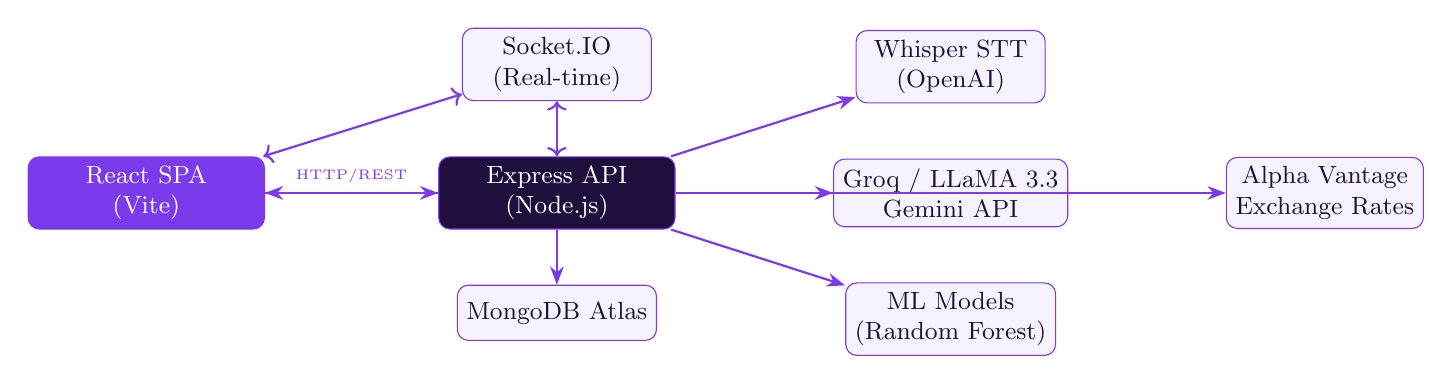
\begin{tikzpicture}[
    node distance=0.7cm and 1.2cm,
    box/.style={rectangle, rounded corners=4pt, minimum width=2.4cm,
                minimum height=0.7cm, align=center, font=\small,
                draw=auraviolet, fill=auragray, text=auradark},
    arrow/.style={-Stealth, thick, color=auraviolet}
  ]
    % Frontend
    \node[box, fill=auraviolet, text=white, minimum width=3cm] (fe) {React SPA\\(Vite)};
    % Backend
    \node[box, fill=auradark, text=white, minimum width=3cm, right=2.2cm of fe] (be) {Express API\\(Node.js)};
    % DB
    \node[box, below=of be] (db) {MongoDB Atlas};
    % Socket
    \node[box, above=of be] (ws) {Socket.IO\\(Real-time)};
    % AI
    \node[box, right=2.0cm of be] (ai) {Groq / LLaMA 3.3\\Gemini API};
    % ML
    \node[box, below=of ai] (ml) {ML Models\\(Random Forest)};
    % STT
    \node[box, above=of ai] (stt) {Whisper STT\\(OpenAI)};
    % Stock
    \node[box, right=2.0cm of ai] (ext) {Alpha Vantage\\Exchange Rates};

    % Arrows
    \draw[arrow] (fe) -- node[above, font=\tiny]{HTTP/REST} (be);
    \draw[arrow] (be) -- (fe);
    \draw[arrow, <->] (fe) -- (ws);
    \draw[arrow, <->] (ws) -- (be);
    \draw[arrow] (be) -- (db);
    \draw[arrow] (be) -- (ai);
    \draw[arrow] (be) -- (ml);
    \draw[arrow] (be) -- (stt);
    \draw[arrow] (be) -- (ext);
  \end{tikzpicture}
  \end{center}
\end{frame}

\begin{frame}{Proposed Solution — Key Features}
  \begin{columns}[T]
    \begin{column}{0.48\textwidth}
      \begin{block}{\faRobot\ \ AI Features}
        \begin{itemize}
          \item \textbf{AI Diary Parser} — describe your day in text/voice; AI extracts all financial events
          \item \textbf{AI Insights} — personalised spending analysis on demand
          \item \textbf{AI Budget Builder} — generates a complete budget from a natural language goal
          \item \textbf{AI Investment Advisor} — stock/crypto suggestions based on profile
        \end{itemize}
      \end{block}
    \end{column}
    \begin{column}{0.48\textwidth}
      \begin{block}{\faUsers\ \ Collaboration \& ML}
        \begin{itemize}
          \item \textbf{Budget Rooms} — shared rooms with real-time transactions, comments, and debt settlements
          \item \textbf{Spending Forecast} — Random Forest model predicts next N days of spending with confidence intervals
          \item \textbf{PDF Reports} — one-click export of full transaction history
          \item \textbf{Multi-currency} — live FX rate support
        \end{itemize}
      \end{block}
    \end{column}
  \end{columns}
\end{frame}

% ============================================================
\section{Technology Stack}
% ============================================================
\begin{frame}{Technology Stack}
  \begin{columns}[T]
    \begin{column}{0.48\textwidth}
      \textbf{Frontend}
      \vspace{4pt}
      \begin{tabularx}{\textwidth}{lX}
        \toprule
        \textbf{Library} & \textbf{Purpose} \\
        \midrule
        React 18 & UI framework \\
        Vite 5 & Build tool / dev server \\
        Axios & HTTP client \\
        Recharts & Charts \& visualisations \\
        Framer Motion & Animations \\
        Socket.IO Client & Real-time events \\
        jsPDF & PDF export \\
        React Router 7 & Client-side routing \\
        \bottomrule
      \end{tabularx}
    \end{column}
    \begin{column}{0.48\textwidth}
      \textbf{Backend \& AI/ML}
      \vspace{4pt}
      \begin{tabularx}{\textwidth}{lX}
        \toprule
        \textbf{Technology} & \textbf{Purpose} \\
        \midrule
        Node.js + Express 5 & REST API server \\
        MongoDB + Mongoose & Database \& ODM \\
        Socket.IO 4 & WebSocket server \\
        JWT + bcryptjs & Auth \& security \\
        Groq SDK (LLaMA 3.3) & LLM insights \\
        Google Gemini API & Secondary LLM \\
        OpenAI Whisper & Voice transcription \\
        Python / scikit-learn & ML model training \\
        Alpha Vantage & Stock data \\
        \bottomrule
      \end{tabularx}
    \end{column}
  \end{columns}
\end{frame}

% ============================================================
\section{Challenges Faced}
% ============================================================
\begin{frame}{Challenges Faced}
  \begin{enumerate}
    \item[\textcolor{auraviolet}{\faExclamationTriangle}] \textbf{LLM Output Parsing} \\
          LLMs occasionally return malformed JSON or extra text. Solved with strict prompt engineering and fallback parsers.

    \vspace{5pt}
    \item[\textcolor{auraviolet}{\faExclamationTriangle}] \textbf{Transaction De-duplication from Diary} \\
          AI-parsed diary entries sometimes created duplicate transactions (e.g., both a purchase and a subscription entry for the same item). Required careful prompt and post-processing logic.

    \vspace{5pt}
    \item[\textcolor{auraviolet}{\faExclamationTriangle}] \textbf{Real-Time State Consistency} \\
          Keeping multiple clients' UI in sync over Socket.IO without race conditions required careful event sequencing.

    \vspace{5pt}
    \item[\textcolor{auraviolet}{\faExclamationTriangle}] \textbf{Multi-Currency Support} \\
          Investment values are fetched in USD (Alpha Vantage); converting and displaying them correctly in the user's preferred currency required live exchange-rate caching.

    \vspace{5pt}
    \item[\textcolor{auraviolet}{\faExclamationTriangle}] \textbf{ML Data Scarcity} \\
          Personal finance datasets are private. Used a Kaggle dataset and seeded mock data to train the Random Forest forecasting model.
  \end{enumerate}
\end{frame}

% ============================================================
\section{Expected Outcomes}
% ============================================================
\begin{frame}{Expected Outcomes}
  \begin{columns}[T]
    \begin{column}{0.48\textwidth}
      \begin{block}{User Benefits}
        \begin{itemize}
          \bulletitem{Reduced time spent on manual expense categorisation through AI-powered diary parsing}
          \bulletitem{Better financial awareness via personalised LLM insights and budget recommendations}
          \bulletitem{Improved savings rates through ML spending forecasts and goal tracking}
          \bulletitem{Seamless shared-expense management for households and groups}
        \end{itemize}
      \end{block}
    \end{column}
    \begin{column}{0.48\textwidth}
      \begin{block}{Technical Outcomes}
        \begin{itemize}
          \bulletitem{A fully-functional, production-ready MERN stack application}
          \bulletitem{Demonstrated integration of multiple LLM APIs within a single application}
          \bulletitem{A trained Random Forest model achieving reasonable accuracy on spending forecasts}
          \bulletitem{A reusable pattern for real-time collaborative finance features using Socket.IO}
        \end{itemize}
      \end{block}
    \end{column}
  \end{columns}

  \vspace{10pt}
  \begin{alertblock}{Broader Impact}
    Aura Budget demonstrates that AI and ML can lower the barrier to financial
    literacy — making smart money management accessible to anyone with a
    smartphone and an internet connection.
  \end{alertblock}
\end{frame}

% ---- Thank You ----
\begin{frame}
  \begin{center}
    \vspace{20pt}
    {\Huge \textcolor{auraviolet}{\textbf{Thank You}}}

    \vspace{20pt}
    {\large Questions \& Discussion}

    \vspace{30pt}
    
\begin{tikzpicture}
      \node[rectangle, rounded corners=8pt, fill=auraviolet, text=white,
            minimum width=6cm, minimum height=1.2cm, font=\large\bfseries]
            {Aura Budget};
    \end{tikzpicture}

    \vspace{15pt}
    \small\textcolor{auradark}{
      AI-Powered Personal Finance Management System \\
      Built with React · Node.js · MongoDB · LLaMA 3.3 · Python/ML
    }
  \end{center}
\end{frame}

\end{document}
